% Options for packages loaded elsewhere
\PassOptionsToPackage{unicode}{hyperref}
\PassOptionsToPackage{hyphens}{url}
%
\documentclass[
]{article}
\usepackage{amsmath,amssymb}
\usepackage{lmodern}
\usepackage{iftex}
\ifPDFTeX
  \usepackage[T1]{fontenc}
  \usepackage[utf8]{inputenc}
  \usepackage{textcomp} % provide euro and other symbols
\else % if luatex or xetex
  \usepackage{unicode-math}
  \defaultfontfeatures{Scale=MatchLowercase}
  \defaultfontfeatures[\rmfamily]{Ligatures=TeX,Scale=1}
\fi
% Use upquote if available, for straight quotes in verbatim environments
\IfFileExists{upquote.sty}{\usepackage{upquote}}{}
\IfFileExists{microtype.sty}{% use microtype if available
  \usepackage[]{microtype}
  \UseMicrotypeSet[protrusion]{basicmath} % disable protrusion for tt fonts
}{}
\makeatletter
\@ifundefined{KOMAClassName}{% if non-KOMA class
  \IfFileExists{parskip.sty}{%
    \usepackage{parskip}
  }{% else
    \setlength{\parindent}{0pt}
    \setlength{\parskip}{6pt plus 2pt minus 1pt}}
}{% if KOMA class
  \KOMAoptions{parskip=half}}
\makeatother
\usepackage{xcolor}
\usepackage[margin=2.54cm]{geometry}
\usepackage{graphicx}
\makeatletter
\def\maxwidth{\ifdim\Gin@nat@width>\linewidth\linewidth\else\Gin@nat@width\fi}
\def\maxheight{\ifdim\Gin@nat@height>\textheight\textheight\else\Gin@nat@height\fi}
\makeatother
% Scale images if necessary, so that they will not overflow the page
% margins by default, and it is still possible to overwrite the defaults
% using explicit options in \includegraphics[width, height, ...]{}
\setkeys{Gin}{width=\maxwidth,height=\maxheight,keepaspectratio}
% Set default figure placement to htbp
\makeatletter
\def\fps@figure{htbp}
\makeatother
\setlength{\emergencystretch}{3em} % prevent overfull lines
\providecommand{\tightlist}{%
  \setlength{\itemsep}{0pt}\setlength{\parskip}{0pt}}
\setcounter{secnumdepth}{-\maxdimen} % remove section numbering
\usepackage{booktabs}
\usepackage{longtable}
\usepackage{array}
\usepackage{multirow}
\usepackage{wrapfig}
\usepackage{float}
\usepackage{colortbl}
\usepackage{pdflscape}
\usepackage{tabu}
\usepackage{threeparttable}
\usepackage{threeparttablex}
\usepackage[normalem]{ulem}
\usepackage{makecell}
\usepackage{xcolor}
\ifLuaTeX
  \usepackage{selnolig}  % disable illegal ligatures
\fi
\IfFileExists{bookmark.sty}{\usepackage{bookmark}}{\usepackage{hyperref}}
\IfFileExists{xurl.sty}{\usepackage{xurl}}{} % add URL line breaks if available
\urlstyle{same} % disable monospaced font for URLs
\hypersetup{
  pdftitle={Winter Is Coming: Forecasting Electricity and Natural Gas Prices for Home Heating},
  pdfauthor={Justin DePue, John Rooney, and Tony Jiang},
  hidelinks,
  pdfcreator={LaTeX via pandoc}}

\title{Winter Is Coming: Forecasting Electricity and Natural Gas Prices
for Home Heating}
\author{Justin DePue, John Rooney, and Tony Jiang}
\date{2023-04-28}

\begin{document}
\maketitle

{
\setcounter{tocdepth}{3}
\tableofcontents
}
\begin{itemize}
\tightlist
\item
  Knitting commands in code chunks:

  \begin{itemize}
  \tightlist
  \item
    \texttt{include\ =\ FALSE} - code is run, but neither code nor
    results appear in knitted file
  \item
    \texttt{echo\ =\ FALSE} - code not included in knitted file, but
    results are
  \item
    \texttt{eval\ =\ FALSE} - code is not run in the knitted file
  \item
    \texttt{message\ =\ FALSE} - messages do not appear in knitted file
  \item
    \texttt{warning\ =\ FALSE} - warnings do not appear\ldots{}
  \item
    \texttt{fig.cap\ =\ "..."} - adds a caption to graphical results
  \end{itemize}
\end{itemize}

\hypertarget{introduction}{%
\subsection{Introduction}\label{introduction}}

This study was born out of both curiosity and necessity. One of our
teammates faced higher than expected energy bills this winter and was
suddenly faced with the question of whether to shiver to save money or
spend it on heating bills and be forced to eat Spaghetti-O's as
sustenance. While spring has sprung and summer is on the horizon, we
know that winter is coming and that we should prepare now in order that
history not repeat itself.

As students recently armed with the tools to conduct time series
analysis and forecasting, we realized we could complete our final
project while aiding our teammate with knowledge for the future. Our
study question thus emerged: would it be more cost-effective to heat an
apartment in North Carolina using electricity or a natural-gas powered
heater?

Full of optimism that we could complete a class requirement while doing
some good for the world (for as Marvel taught us, when you help someone,
you help everyone), we set out to find the data that would lead us to
the answer we sought. Our journey led us to that great repository of
energy knowledge, the US Energy Information Administration. There we
found two datasets we felt confident would help us help our teammate:
``North Carolina Price of Natural Gas Delivered to Residential Customers
(Dollars Per Thousand Cubic Feet)'', which contained monthly data from
January 1989 through January 2023, and ``Average Retail Price of
Electricity by State and Sector'' which contained monthly data from
January 2001 through January 2023.

\hypertarget{data}{%
\subsection{Data}\label{data}}

Both datasets were downloaded from the EIA as .csv files. The most
significant data wrangling was done with the natural gas data as it was
originally provided in dollars per thousand cubic feet and needed to be
in dollars per kilowatt hour for comparison with electricity data. The
electricity data was provided monthly for both regions and states by
sector. The natural gas data was provided monthly for North Carolina
accompanied by price.

\begin{table}[H]

\caption{\label{tab:unnamed-chunk-1}Table 1: Summary Statistics}
\centering
\begin{tabular}[t]{l|r|r|r|r|r|r}
\hline
Variable & Observations & Min & Max & Mean Price & Std. Dev. & Median Price\\
\hline
\cellcolor{gray!6}{Natural Gas (\$/Mcf)} & \cellcolor{gray!6}{410} & \cellcolor{gray!6}{5.54} & \cellcolor{gray!6}{30.43} & \cellcolor{gray!6}{13.78} & \cellcolor{gray!6}{5.64} & \cellcolor{gray!6}{12.54}\\
\hline
Electricity(cents/kWh) & 265 & 7.53 & 13.51 & 10.22 & 1.30 & 10.41\\
\hline
\end{tabular}
\end{table}

\begin{table}[H]

\caption{\label{tab:unnamed-chunk-2}Sample of Cleaned Natural Gas Data}
\centering
\begin{tabular}[t]{l|r}
\hline
year & price\\
\hline
\cellcolor{gray!6}{Jan-1989} & \cellcolor{gray!6}{6.17}\\
\hline
Feb-1989 & 6.30\\
\hline
\cellcolor{gray!6}{Mar-1989} & \cellcolor{gray!6}{6.29}\\
\hline
Apr-1989 & 6.80\\
\hline
\cellcolor{gray!6}{May-1989} & \cellcolor{gray!6}{6.99}\\
\hline
Jun-1989 & 8.02\\
\hline
\cellcolor{gray!6}{Jul-1989} & \cellcolor{gray!6}{8.71}\\
\hline
Aug-1989 & 8.97\\
\hline
\cellcolor{gray!6}{Sep-1989} & \cellcolor{gray!6}{8.68}\\
\hline
Oct-1989 & 7.44\\
\hline
\end{tabular}
\end{table}

\begin{table}[H]

\caption{\label{tab:unnamed-chunk-2}Sample of Cleaned Electricity Data}
\centering
\begin{tabular}[t]{l|r}
\hline
my\_date & price\_per\_kWh\\
\hline
\cellcolor{gray!6}{Jan.2001} & \cellcolor{gray!6}{7.53}\\
\hline
Feb.2001 & 7.77\\
\hline
\cellcolor{gray!6}{Mar.2001} & \cellcolor{gray!6}{8.02}\\
\hline
Apr.2001 & 8.00\\
\hline
\cellcolor{gray!6}{May.2001} & \cellcolor{gray!6}{8.22}\\
\hline
Jun.2001 & 8.19\\
\hline
\cellcolor{gray!6}{Jul.2001} & \cellcolor{gray!6}{8.31}\\
\hline
Aug.2001 & 8.35\\
\hline
\cellcolor{gray!6}{Sep.2001} & \cellcolor{gray!6}{8.35}\\
\hline
Oct.2001 & 8.67\\
\hline
\end{tabular}
\end{table}

\hypertarget{analysis}{%
\subsection{Analysis}\label{analysis}}

Our analysis began by creating initial time series objects and plotting
them, along with creating ACF and PACF plots to gain an initial sense of
what the series looked like and what seasonality they may have.

We then decomposed the time series objects for further analysis to
visualize the trend and seasonality of each series. The decomposition of
the natural gas time series object shows clear seasonality in price
along with a steep upward trend beginning in 2020. The decomposition of
electricity prices shows a clear upward trend from the beginning of the
series and shows a bimodal seasonality.

\includegraphics{Final-Project_files/figure-latex/plot elec and gas ts-1.pdf}

\includegraphics{Final-Project_files/figure-latex/decompose ts-1.pdf}
\includegraphics{Final-Project_files/figure-latex/decompose ts-2.pdf}

\includegraphics{Final-Project_files/figure-latex/ACF and PACF of electricity and natural gas-1.pdf}
\includegraphics{Final-Project_files/figure-latex/ACF and PACF of electricity and natural gas-2.pdf}
\includegraphics{Final-Project_files/figure-latex/ACF and PACF of electricity and natural gas-3.pdf}
\includegraphics{Final-Project_files/figure-latex/ACF and PACF of electricity and natural gas-4.pdf}

Several models were developed and tested to determine what would best
fit the data we had and what may lead to the best forecast to determine
whether heating via electricity or natural gas would be most
cost-efficient in the upcoming winter. The five that were used were the
Seasonal ARIMA, ARIMA with Fourier terms, Neural Networks, TBATS, and
STL + EST.

Each of these tests used functions from the ``forecast'' library and
required the use of time series data which we created using the ``ts''
function from the ``tseries'' library.

While the Seasonal ARIMA was a logical first model to try, we quickly
felt that the performance was not particularly strong and that
developing and testing other models was warranted.

\includegraphics{Final-Project_files/figure-latex/Seasonal Arima-1.pdf}
\includegraphics{Final-Project_files/figure-latex/Seasonal Arima-2.pdf}

We decided to explore more advanced models such as the ARIMA with
Fourier Terms model, Neural Networks, TBATS, and STL + EST. ARIMA with
Fourier terms is known as a dynamic harmonic regression model with an
ARMA error structure, using the ``fourier'' function from package
``forecast'' to find terms that model seasonal components.

\includegraphics{Final-Project_files/figure-latex/Arima with Fourier terms-1.pdf}
\includegraphics{Final-Project_files/figure-latex/Arima with Fourier terms-2.pdf}

~ ~

We next developed and tested an STL model.

~ ~ \includegraphics{Final-Project_files/figure-latex/STL -1.pdf}
\includegraphics{Final-Project_files/figure-latex/STL -2.pdf}

~ ~

We then developed and test a neural network model using the ``nnetar()''
function in the ``forecast'' package. We learned that the p and P
arguments in nnetar() have significant impact on model performance.
Therefore, we worked to identify the optimal p and P combination through
trial and error.

~ ~

\begin{table}[H]

\caption{\label{tab:unnamed-chunk-6}Natural Gas Neural Net Forecast Accuracy using Various Seasonal Lag Inputs (p/P)}
\centering
\begin{tabular}[t]{l|r|r|r|r|r|r|r}
\hline
  & ME & RMSE & MAE & MPE & MAPE & ACF1 & Theil's U\\
\hline
\cellcolor{gray!6}{1/0} & \cellcolor{gray!6}{-1.17533} & \cellcolor{gray!6}{1.29899} & \cellcolor{gray!6}{1.17533} & \cellcolor{gray!6}{-10.54275} & \cellcolor{gray!6}{10.54275} & \cellcolor{gray!6}{0.28462} & \cellcolor{gray!6}{46.21817}\\
\hline
1/1 & -0.87616 & 0.98800 & 0.87616 & -7.63726 & 7.63726 & 0.18467 & 4.68394\\
\hline
\cellcolor{gray!6}{2/0} & \cellcolor{gray!6}{-1.01868} & \cellcolor{gray!6}{1.14866} & \cellcolor{gray!6}{1.01868} & \cellcolor{gray!6}{-9.00372} & \cellcolor{gray!6}{9.00372} & \cellcolor{gray!6}{0.29337} & \cellcolor{gray!6}{17.28475}\\
\hline
2/1 & -0.88198 & 0.99880 & 0.88198 & -7.69491 & 7.69491 & 0.21716 & 4.89079\\
\hline
\cellcolor{gray!6}{2/2} & \cellcolor{gray!6}{-0.87055} & \cellcolor{gray!6}{0.99976} & \cellcolor{gray!6}{0.87055} & \cellcolor{gray!6}{-7.60248} & \cellcolor{gray!6}{7.60248} & \cellcolor{gray!6}{0.22890} & \cellcolor{gray!6}{4.45841}\\
\hline
1/2 & -0.87183 & 0.99579 & 0.87183 & -7.60606 & 7.60606 & 0.20963 & 4.84902\\
\hline
\cellcolor{gray!6}{3/1} & \cellcolor{gray!6}{-0.89269} & \cellcolor{gray!6}{1.00988} & \cellcolor{gray!6}{0.89269} & \cellcolor{gray!6}{-7.79637} & \cellcolor{gray!6}{7.79637} & \cellcolor{gray!6}{0.22178} & \cellcolor{gray!6}{4.99201}\\
\hline
\end{tabular}
\end{table}

\begin{table}[H]

\caption{\label{tab:unnamed-chunk-7}Natural Gas Neural Net Forecast Accuracy using Various Seasonal Lag Inputs (p/P)}
\centering
\begin{tabular}[t]{l|r|r|r|r|r|r|r}
\hline
  & ME & RMSE & MAE & MPE & MAPE & ACF1 & Theil's U\\
\hline
\cellcolor{gray!6}{1/0} & \cellcolor{gray!6}{-2.29022} & \cellcolor{gray!6}{3.00280} & \cellcolor{gray!6}{2.39520} & \cellcolor{gray!6}{-33.52580} & \cellcolor{gray!6}{34.93346} & \cellcolor{gray!6}{0.62860} & \cellcolor{gray!6}{18.47359}\\
\hline
1/1 & -1.78745 & 2.24463 & 1.97096 & -25.51708 & 27.72316 & 0.29670 & 2.46832\\
\hline
\cellcolor{gray!6}{2/0} & \cellcolor{gray!6}{-2.50531} & \cellcolor{gray!6}{3.28770} & \cellcolor{gray!6}{2.68980} & \cellcolor{gray!6}{-40.09569} & \cellcolor{gray!6}{42.43958} & \cellcolor{gray!6}{0.67398} & \cellcolor{gray!6}{12.26527}\\
\hline
2/1 & -1.86549 & 2.20039 & 1.93552 & -27.02312 & 27.76145 & 0.22357 & 2.49269\\
\hline
\cellcolor{gray!6}{2/2} & \cellcolor{gray!6}{-2.02121} & \cellcolor{gray!6}{2.35638} & \cellcolor{gray!6}{2.06264} & \cellcolor{gray!6}{-30.01317} & \cellcolor{gray!6}{30.45799} & \cellcolor{gray!6}{0.27527} & \cellcolor{gray!6}{2.72891}\\
\hline
1/2 & -1.90493 & 2.31009 & 1.97513 & -27.51662 & 28.25710 & 0.27918 & 2.59018\\
\hline
\cellcolor{gray!6}{3/1} & \cellcolor{gray!6}{-1.94234} & \cellcolor{gray!6}{2.27873} & \cellcolor{gray!6}{1.99919} & \cellcolor{gray!6}{-28.62680} & \cellcolor{gray!6}{29.23123} & \cellcolor{gray!6}{0.27015} & \cellcolor{gray!6}{2.61629}\\
\hline
3/2 & -1.90516 & 2.23854 & 1.96266 & -27.98058 & 28.59165 & 0.26164 & 2.56135\\
\hline
\cellcolor{gray!6}{33} & \cellcolor{gray!6}{-2.02602} & \cellcolor{gray!6}{2.34778} & \cellcolor{gray!6}{2.11605} & \cellcolor{gray!6}{-30.45846} & \cellcolor{gray!6}{31.39579} & \cellcolor{gray!6}{0.19397} & \cellcolor{gray!6}{2.48299}\\
\hline
\end{tabular}
\end{table}

~ ~

We found that combination 11 (p = 1 and P = 1) had the best modeling
performance for our electricity series, and combination 32 (p = 3 and P
= 2) had the best modeling performance for our natural gas series. We
then used combination 11 to run a neural network model with fourier
terms for our electricity series.

~ ~
\includegraphics{Final-Project_files/figure-latex/unnamed-chunk-8-1.pdf}
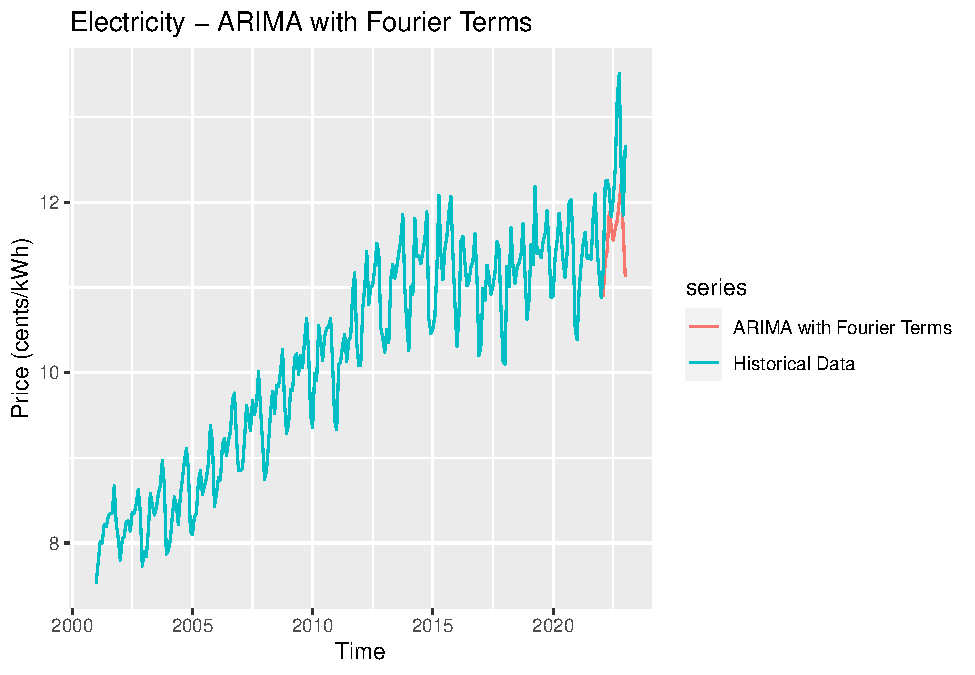
\includegraphics{Final-Project_files/figure-latex/unnamed-chunk-9-1.pdf}

~ ~

We then developed and tested a TBATS models for our electricity and
natural gas series.

~ ~

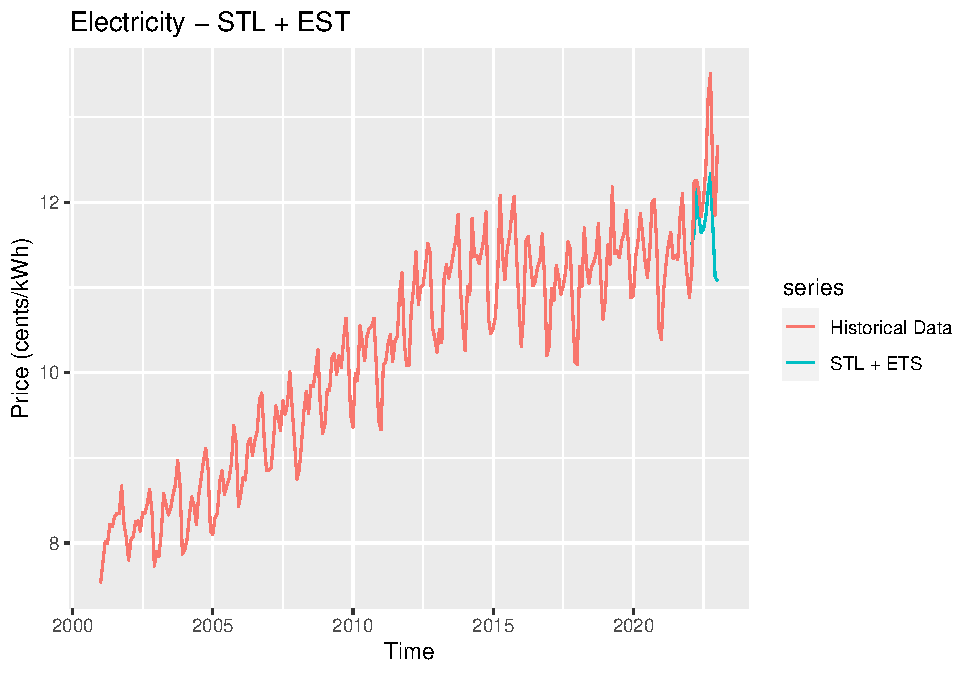
\includegraphics{Final-Project_files/figure-latex/unnamed-chunk-11-1.pdf}

~ ~

\includegraphics{Final-Project_files/figure-latex/unnamed-chunk-12-1.pdf}
~ ~

~ ~ As we thought about other ways to model our time series, we realized
that the Ukraine War has had a significant impact on natural gas prices,
and likely eletricity price, too. We additionally realized temperature
would be a good regressor to include since utility bills normally
fluctuate in the same direction as temperature. Therefore, we created
two covariates: UKRWAR and temperature. \(UKRWAR\) is an indicator
variable with values of 0 and 1. Months before March 2022 have a value
of 0, while months after and including March 2022 have a value of 1. The
reason why we set the cutoff month at March 2022 despite the war
starting in February of that year is because the impact of the war on
monthly natural gas prices in February 2022 should be limited because of
the war beginning that month. The temperature series is the monthly
average temperature of the Raleigh area. This is largest geographic
level of historical temperature data. ~ ~

~ ~

After creating all the covariates, we repeated our modeling but with
covariates to improve the accuracy of the models. First we incorporated
covariates into our neural network model.

~ ~

\includegraphics{Final-Project_files/figure-latex/unnamed-chunk-15-1.pdf}

~ ~
\includegraphics{Final-Project_files/figure-latex/unnamed-chunk-16-1.pdf}

~ ~

~ ~

We then developed a seasonal arima model with temperature and fourier
terms to model two series. UKRWAR as a covariate was excluded because R
reported no suitable ARIMA model when UKRWAR was included. The function
used for this was ``auto.arima(xreg)''.

~ ~

\includegraphics{Final-Project_files/figure-latex/unnamed-chunk-18-1.pdf}

~ ~
\includegraphics{Final-Project_files/figure-latex/unnamed-chunk-19-1.pdf}

~ ~

~ ~

\hypertarget{summary-and-conclusions}{%
\subsection{Summary and Conclusions}\label{summary-and-conclusions}}

When comparing the accuracy of each of the models that were tested, the
STL model emerged as the best fit for both the price of electricity and
the price of natural gas when comparing both the RMSE and MAPE scores.
Both models missed the heights seen in 2022, however. There could be
several reasons for this. One is the difficulty of modeling for the
beginning of the war in Ukraine and the impact that has had on natural
gas prices both regionally and around the world. Another is the
difficulty of modeling for the influence of generationally high
inflation. With both of these compounding each other, it is perhaps not
surprising that all of the models failed to predict the rise in price
for both electricity and natural gas.

~ ~

\includegraphics{Final-Project_files/figure-latex/compare performace scores and generate tables for use-1.pdf}
\includegraphics{Final-Project_files/figure-latex/compare performace scores and generate tables for use-2.pdf}

\begin{verbatim}
## The best model for electricity by RMSE is:  STL
\end{verbatim}

\begin{table}[!h]

\caption{\label{tab:compare performace scores and generate tables for use}Forecast Accuracy for NC Residential Electricity Price}
\centering
\begin{tabular}[t]{l|r|r|r|r|r|r|r}
\hline
  & ME & RMSE & MAE & MPE & MAPE & ACF1 & Theil's U\\
\hline
SARIMA & -0.67702 & 0.83764 & 0.70998 & -5.83726 & 6.12612 & 0.25988 & 2.73983\\
\hline
ARIMA with Fourier & -0.69902 & 0.87542 & 0.69902 & -6.04752 & 6.04752 & 0.08221 & 2.82856\\
\hline
\cellcolor{red}{STL} & \cellcolor{red}{-0.58551} & \cellcolor{red}{0.76708} & \cellcolor{red}{0.63447} & \cellcolor{red}{-5.01390} & \cellcolor{red}{5.43949} & \cellcolor{red}{0.25835} & \cellcolor{red}{2.36056}\\
\hline
Neural Network & -1.04081 & 1.20229 & 1.04081 & -9.32361 & 9.32361 & 0.16593 & 2.98616\\
\hline
TBATS & -0.74971 & 0.89063 & 0.75658 & -6.50522 & 6.56626 & 0.23462 & 2.86546\\
\hline
Neural Network with Covariates & -0.93643 & 1.11078 & 0.96737 & -8.33578 & 8.60733 & 0.42834 & 2.60972\\
\hline
SARIMA with Tem and Fourier & -0.67930 & 0.81795 & 0.69585 & -5.83257 & 5.97891 & 0.26220 & 2.92123\\
\hline
\end{tabular}
\end{table}

\begin{verbatim}
## The best model for natural gas by RMSE is:  STL
\end{verbatim}

\begin{table}[!h]

\caption{\label{tab:compare performace scores and generate tables for use}Forecast Accuracy for NC Residential Natural Gas Price}
\centering
\begin{tabular}[t]{l|r|r|r|r|r|r|r}
\hline
  & ME & RMSE & MAE & MPE & MAPE & ACF1 & Theil's U\\
\hline
SARIMA & -1.67902 & 1.97784 & 1.67902 & -23.35174 & 23.35174 & -0.15535 & 1.81675\\
\hline
ARIMA with Fourier & -1.73518 & 2.31200 & 1.83981 & -25.17044 & 26.24995 & 0.57850 & 3.12541\\
\hline
\cellcolor{red}{STL} & \cellcolor{red}{-1.04788} & \cellcolor{red}{1.35599} & \cellcolor{red}{1.11314} & \cellcolor{red}{-14.03428} & \cellcolor{red}{14.80904} & \cellcolor{red}{-0.33348} & \cellcolor{red}{1.28849}\\
\hline
Neural Network & -1.84141 & 2.19912 & 1.90132 & -26.85398 & 27.48965 & 0.46790 & 2.70025\\
\hline
TBATS & -1.72858 & 1.89245 & 1.72858 & -24.53539 & 24.53539 & -0.32231 & 2.08610\\
\hline
Neural Network with Covariates & -1.20788 & 1.74944 & 1.47158 & -15.02970 & 18.27107 & 0.49787 & 2.20138\\
\hline
SARIMA with Tem and Fourier & -1.63275 & 1.79495 & 1.63275 & -21.52016 & 21.52016 & -0.01071 & 1.95240\\
\hline
\end{tabular}
\end{table}

~ ~

Our initial research question posed how our roommate could best plan for
surviving, if not thriving, in the upcoming winter. Based on our
analysis, the answer appears to be that he would be best off by buying a
natural gas-powered heater. Given the vicissitudes of energy prices seen
in recent months, and the uncertainty of global and domestic events that
could further impact energy prices, this is hard to say with certainty.
Revisiting these forecasts both ahead of the upcoming winter and
annually thereafter with updated data would be well-advised.

\includegraphics{Final-Project_files/figure-latex/unnamed-chunk-22-1.pdf}

\end{document}
